\documentclass[journal, onecolumn]{IEEEtran}

% --- PACKAGES ---
\usepackage{amsmath}
\usepackage{amssymb}
\usepackage{amsfonts}
\usepackage{amsthm}
\usepackage{graphicx}
\usepackage[utf8]{inputenc}
\usepackage[T1]{fontenc}
\usepackage{url}
\usepackage{xcolor}
\usepackage{framed}
\usepackage{enumitem}
\usepackage{tcolorbox}
\usepackage{tikz}
\usepackage{float}
\usetikzlibrary{arrows.meta, positioning, shapes.geometric, calc, decorations.pathreplacing}

% --- USER PREFERENCE COLORS ---
\definecolor{Garnet}{HTML}{73000a}
\definecolor{SecondaryBlue}{HTML}{466A9F}
\definecolor{SecondaryGreen}{HTML}{65780B}
\definecolor{FlatRed}{HTML}{CC2E40}
\definecolor{FlatDark}{HTML}{1F414D}
\definecolor{FlatYellow}{HTML}{CED318}
\definecolor{FlatGold}{HTML}{A49137}
\definecolor{LightGray}{HTML}{F0F0F0}

% --- FORMATTING ---
\setlength{\parindent}{0pt}
\setlength{\parskip}{1.2em}
\renewcommand{\baselinestretch}{1.2}

% --- CUSTOM COMMANDS ---
\newcommand{\vocab}[1]{\textbf{\textcolor{Garnet}{#1}}}
\newcommand{\mathhighlight}[1]{\textcolor{SecondaryBlue}{#1}}

% --- TCOLORBOX STYLES ---
\tcbset{
    examplebox/.style={
        colback=LightGray,
        colframe=SecondaryBlue,
        fonttitle=\bfseries,
        title=#1,
        sharp corners,
        boxrule=1pt
    },
    memorybox/.style={
        colback=Garnet!10,
        colframe=Garnet,
        fonttitle=\bfseries,
        title=#1,
        sharp corners,
        boxrule=2pt
    }
}

% --- TITLE & AUTHOR ---
\title{\textcolor{Garnet}{\textbf{The Bellman Equation: A Comprehensive Guide}}}
\author{A Step-by-Step Derivation with Practical Examples}
\date{\today}

\begin{document}

\maketitle

\begin{abstract}
This document provides a complete derivation of the Bellman Equation using a \textbf{single running example}: a pizza delivery driver navigating a city. Every concept is illustrated with concrete numbers you can trace through by hand. By the end, you'll understand not just \textit{what} the Bellman Equation says, but \textit{why} it must be true.
\end{abstract}

% ==========================================
\section{Part 1: The Big Picture}
% ==========================================

\subsection{The Problem We're Solving}

You're a pizza delivery driver. You have a map of the city with different intersections. Your goal: figure out which route maximizes your tips over your entire shift.

\begin{tcolorbox}[memorybox={The Core Question}]
\textbf{If I'm standing at this intersection right now, how much money will I make from here until I clock out?}

This number---the total expected future earnings from a location---is called the \vocab{Value} of that location.
\end{tcolorbox}

Here's the insight that makes the Bellman Equation powerful:

\textit{You don't need to simulate your entire future to know how good your current spot is. You only need to know:}
\begin{enumerate}
    \item What you'll earn in the \textbf{next few minutes} (immediate reward)
    \item How good the \textbf{next intersection} is (and you can look that up!)
\end{enumerate}

\begin{figure}[H]
    \centering
    
\begin{tikzpicture}[node distance=5.5cm, thick]
        % Nodes
        \node[draw=none, fill=Garnet, text=white, minimum width=3cm, minimum height=1.5cm] (agent) {\textbf{Driver (Agent)}};
        \node[draw=none, fill=SecondaryBlue, text=white, minimum width=3cm, minimum height=1.5cm, right=of agent] (env) {\textbf{City (Environment)}};

        % Arrows
        \draw[-{Latex[length=3mm]}, FlatDark, line width=1.5pt] ([yshift=0.4cm]agent.east) -- node[above, font=\small\bfseries] {Drive to $A_t$} ([yshift=0.4cm]env.west);
        \draw[-{Latex[length=3mm]}, FlatDark, line width=1.5pt] ([yshift=-0.4cm]env.west) -- node[below, font=\small\bfseries] {New location $S_{t+1}$, Tip $R_{t+1}$} ([yshift=-0.4cm]agent.east);
    \end{tikzpicture}
    \caption{The RL Loop: You (the agent) pick a route. The city (environment) gives you a new location and a tip.}
    \label{fig:rl_loop}
\end{figure}

\newpage
% ==========================================
\section{Part 2: The Vocabulary with Numbers}
% ==========================================

We'll define every term using our pizza delivery scenario, with \textbf{actual numbers} you can follow.

\subsection{State: $s$ --- ``Where Am I?''}

\begin{tcolorbox}[examplebox={Pizza Delivery Map}]
Imagine the city has 4 key locations:
\begin{itemize}
    \item $s_A$ = Downtown (lots of apartments, good tips)
    \item $s_B$ = Suburbs (far drives, okay tips)
    \item $s_C$ = University (students tip poorly but order often)
    \item $s_D$ = Restaurant (home base, no deliveries here)
\end{itemize}
\textbf{Your state is your current location.} If you're downtown, $S_t = s_A$.
\end{tcolorbox}

\subsection{Reward: $R_{t+1}$ --- ``What Did I Just Earn?''}

The reward is the \textbf{immediate payoff} after you take an action.

\begin{tcolorbox}[examplebox={Concrete Tip Values}]
\begin{itemize}
    \item Deliver downtown ($s_A$): Tip = \$8
    \item Deliver to suburbs ($s_B$): Tip = \$5
    \item Deliver to university ($s_C$): Tip = \$3
    \item Sitting at restaurant ($s_D$): Tip = \$0
\end{itemize}
Note: We write $R_{t+1}$ (not $R_t$) because you receive the tip \textit{after} completing the delivery.
\end{tcolorbox}

\subsection{Return: $G_t$ --- ``My Total Earnings''}

The \vocab{Return} is the sum of ALL future tips from now until you clock out.

\begin{tcolorbox}[examplebox={A Sample Shift}]
Suppose your remaining shift goes: Downtown $\rightarrow$ Suburbs $\rightarrow$ University $\rightarrow$ Done.

Your tips would be: \$8 + \$5 + \$3 = \$16

So if you're currently at the restaurant about to start this route:
\[ G_t = R_{t+1} + R_{t+2} + R_{t+3} = 8 + 5 + 3 = 16 \]
\end{tcolorbox}

\subsection{Discount Factor: $\gamma$ --- ``A Dollar Today vs. Tomorrow''}

Here's a twist: money \textbf{now} is worth more than money \textbf{later}. Why?
\begin{itemize}
    \item You might get in an accident and never collect later tips
    \item You could invest today's money
    \item There's uncertainty about the future
\end{itemize}

We capture this with $\gamma$ (gamma), a number between 0 and 1.

\begin{tcolorbox}[examplebox={The \$100 Test}]
Would you rather have:
\begin{itemize}
    \item[(A)] \$100 right now, or
    \item[(B)] \$100 one hour from now?
\end{itemize}

Most people pick (A). If you're \textit{indifferent} between \$100 now and \$X in an hour, then:
\[ \gamma = \frac{100}{X} \]

If you need \$111 later to feel indifferent, then $\gamma = 100/111 \approx 0.9$.
\end{tcolorbox}

\begin{tcolorbox}[memorybox={Discounted Return Formula}]
\[ G_t = R_{t+1} + \gamma R_{t+2} + \gamma^2 R_{t+3} + \gamma^3 R_{t+4} + \cdots \]

With $\gamma = 0.9$ and tips of \$8, \$5, \$3:
\begin{align*}
G_t &= 8 + (0.9)(5) + (0.9)^2(3) \\
&= 8 + 4.50 + 2.43 \\
&= \$14.93
\end{align*}
Notice: The \$3 tip (two steps away) only contributes \$2.43 to today's value.
\end{tcolorbox}

\begin{figure}[H]
    \centering
    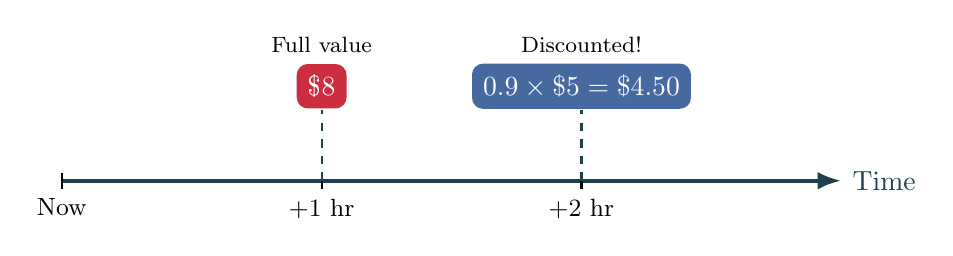
\begin{tikzpicture}[x=2.2cm, y=1cm, thick]
        % Timeline Line
        \draw[->, -{Latex[length=3mm]}, FlatDark, line width=1.5pt] (0,0) -- (4.5,0) node[right] {Time};

        % Ticks
        \foreach \x/\t in {0/Now, 1.5/+1 hr, 3/+2 hr} {
            \draw (\x,0.1) -- (\x,-0.1) node[below] {\small \t};
        }

        % Rewards with actual values
        \node[fill=FlatRed, text=white, inner sep=4pt, rounded corners] at (1.5, 1.2) {\$8};
        \node[fill=SecondaryBlue, text=white, inner sep=4pt, rounded corners] at (3, 1.2) {$0.9 \times \$5 = \$4.50$};

        \draw[dashed, FlatDark] (1.5, 0) -- (1.5, 0.9);
        \draw[dashed, FlatDark] (3, 0) -- (3, 0.9);

        % Labels
        \node[above, font=\footnotesize] at (1.5, 1.5) {Full value};
        \node[above, font=\footnotesize] at (3, 1.5) {Discounted!};

    \end{tikzpicture}
    \caption{Future rewards shrink. A \$5 tip one hour from now is only worth \$4.50 in ``today dollars.''}
    \label{fig:timeline}
\end{figure}

\subsection{Value Function: $v(s)$ --- ``How Good Is This Spot?''}

\begin{tcolorbox}[memorybox={Definition of Value}]
\[ v(s) = \mathbb{E}[G_t \mid S_t = s] \]
\textbf{Translation}: ``The average total money I'll make if I start at location $s$.''
\end{tcolorbox}

\begin{tcolorbox}[examplebox={Intuition Check}]
Which location has higher value?
\begin{itemize}
    \item Downtown ($s_A$): High tips, more orders nearby
    \item University ($s_C$): Low tips, but you might get lucky
\end{itemize}

Clearly $v(s_A) > v(s_C)$. The Bellman equation will let us compute \textit{exactly} how much higher.
\end{tcolorbox}

\newpage
% ==========================================
\section{Part 3: The Math Tools You Need}
% ==========================================

\subsection{Expectation $\mathbb{E}[\cdot]$ = Weighted Average}

When outcomes are random, we compute the \textbf{average} weighted by probability.

\begin{tcolorbox}[examplebox={Traffic Light Example}]
You're approaching an intersection.
\begin{itemize}
    \item 70\% chance: Green light $\rightarrow$ you save 2 minutes
    \item 30\% chance: Red light $\rightarrow$ you lose 1 minute
\end{itemize}

\textbf{Expected time saved}:
\[ \mathbb{E}[\text{time}] = (0.70)(+2) + (0.30)(-1) = 1.4 - 0.3 = +1.1 \text{ minutes} \]

You can't actually save exactly 1.1 minutes, but \textit{on average}, this intersection helps you.
\end{tcolorbox}

\subsection{Linearity of Expectation}

This rule is incredibly useful: \textbf{the average of a sum equals the sum of the averages}.

\[ \mathbb{E}[A + B] = \mathbb{E}[A] + \mathbb{E}[B] \]

\begin{tcolorbox}[examplebox={Why This Matters}]
If your shift has two deliveries:
\begin{itemize}
    \item Expected tip from delivery 1: \$6
    \item Expected tip from delivery 2: \$4
\end{itemize}
Then your expected total is $\mathbb{E}[\text{total}] = 6 + 4 = \$10$.

You don't need to consider all combinations of outcomes!
\end{tcolorbox}

\newpage
% ==========================================
\section{Part 4: The Derivation (With Numbers!)}
% ==========================================

We will derive the Bellman Equation in 6 steps. Here's the roadmap:

\begin{tcolorbox}[memorybox={Derivation Roadmap}]
\begin{enumerate}[leftmargin=*, itemsep=0pt]
    \item \textbf{Start} with the definition of value (total future earnings)
    \item \textbf{Split} into ``now'' and ``later''
    \item \textbf{Separate} the immediate reward from the future
    \item \textbf{Handle uncertainty} about where we go next
    \item \textbf{Recognize} that the future value IS the value function
    \item \textbf{Combine} everything into one beautiful equation
\end{enumerate}
\end{tcolorbox}

\subsection{Setup: Our Running Example}

Throughout this derivation, we'll use a concrete example with real numbers.

\begin{figure}[H]
    \centering
    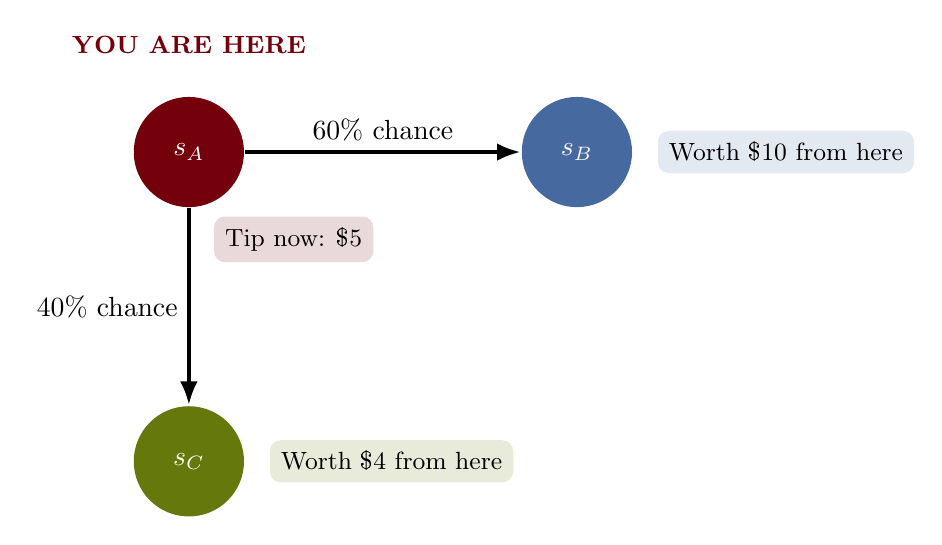
\begin{tikzpicture}[thick, node distance=3.5cm]
        % States
        \node[circle, fill=Garnet, text=white, minimum size=1.4cm] (A) {$s_A$};
        \node[circle, fill=SecondaryBlue, text=white, minimum size=1.4cm, right=of A] (B) {$s_B$};
        \node[circle, fill=SecondaryGreen, text=white, minimum size=1.4cm, below=2.5cm of A] (C) {$s_C$};

        % Arrows with probabilities
        \draw[-{Latex[length=3mm]}, line width=1.5pt] (A) -- node[above] {60\% chance} (B);
        \draw[-{Latex[length=3mm]}, line width=1.5pt] (A) -- node[left] {40\% chance} (C);

        % Value labels
        \node[right=0.3cm of B, font=\small, fill=SecondaryBlue!15, inner sep=4pt, rounded corners] {Worth \$10 from here};
        \node[right=0.3cm of C, font=\small, fill=SecondaryGreen!15, inner sep=4pt, rounded corners] {Worth \$4 from here};

        % Current state label
        \node[above=0.4cm of A, font=\small\bfseries, text=Garnet] {YOU ARE HERE};
        \node[below right=0.3cm and -0.2cm of A, font=\small, fill=Garnet!15, inner sep=4pt, rounded corners] {Tip now: \$5};
    \end{tikzpicture}
    \caption{Our example: You're at $s_A$. You get \$5 immediately, then randomly go to $s_B$ or $s_C$.}
    \label{fig:tiny_city}
\end{figure}

\begin{tcolorbox}[examplebox={The Numbers We'll Use}]
\begin{center}
\renewcommand{\arraystretch}{1.3}
\begin{tabular}{ll}
\textbf{What we know:} & \\
\quad Immediate tip at $s_A$: & $r(s_A) = \$5$ \\
\quad Chance of going to $s_B$: & $p(s_B|s_A) = 0.6$ (60\%) \\
\quad Chance of going to $s_C$: & $p(s_C|s_A) = 0.4$ (40\%) \\
\quad Value of $s_B$ (already computed): & $v(s_B) = \$10$ \\
\quad Value of $s_C$ (already computed): & $v(s_C) = \$4$ \\
\quad Discount factor: & $\gamma = 0.9$ \\[0.5em]
\textbf{What we want to find:} & $v(s_A) = $ ???
\end{tabular}
\end{center}
\end{tcolorbox}

\newpage
\subsection{Step 1: Start with the Definition}

\textbf{The question we're answering}: ``How much money will I make in total if I start at state $s$?''

The value function $v(s)$ is defined as the \textit{expected} total future earnings:

\begin{framed}
\centering
\[ v(s) = \mathbb{E}[\text{Total future earnings} \mid \text{Starting at } s] = \mathbb{E}[G_t \mid S_t = s] \]
\end{framed}

Remember, the total earnings $G_t$ is the sum of all future rewards (with discounting):
\[ G_t = R_{t+1} + \gamma R_{t+2} + \gamma^2 R_{t+3} + \cdots \]

So we can write:
\[ v(s) = \mathbb{E}[\, \underbrace{R_{t+1} + \gamma R_{t+2} + \gamma^2 R_{t+3} + \cdots}_{G_t} \mid S_t = s \,] \]

\begin{tcolorbox}[examplebox={What This Means for $s_A$}]
We want to find: ``If I'm at location $s_A$, what's my expected total earnings?''

This includes:
\begin{itemize}[itemsep=0pt]
    \item The \$5 tip I get right now
    \item Plus all the (discounted) tips I'll get in the future
\end{itemize}
\end{tcolorbox}

\vspace{1em}
\subsection{Step 2: Split ``Now'' vs ``Later''}

Here's the key trick. Let's separate the \textbf{first reward} from \textbf{everything else}:

\[ v(s) = \mathbb{E}[\,\underbrace{R_{t+1}}_{\text{first tip}} + \underbrace{\gamma R_{t+2} + \gamma^2 R_{t+3} + \cdots}_{\text{all future tips}} \mid S_t = s\,] \]

Now, factor out $\gamma$ from the ``future tips'' part:

\[ v(s) = \mathbb{E}[\,R_{t+1} + \gamma \underbrace{(R_{t+2} + \gamma R_{t+3} + \gamma^2 R_{t+4} + \cdots)}_{\text{This looks familiar...}} \mid S_t = s\,] \]

\begin{tcolorbox}[memorybox={The Magic Recognition}]
Look at $(R_{t+2} + \gamma R_{t+3} + \gamma^2 R_{t+4} + \cdots)$.

This is the total return starting from time $t+1$. That's just $G_{t+1}$!

\textbf{Pattern}: $G_t = R_{t+1} + \gamma G_{t+1}$

\textit{``Today's total = today's reward + discounted tomorrow's total''}
\end{tcolorbox}

Substituting $G_{t+1}$:
\begin{equation}
    v(s) = \mathbb{E}[\,R_{t+1} + \gamma G_{t+1} \mid S_t = s\,]
    \label{eq:step2}
\end{equation}

\begin{tcolorbox}[examplebox={Pizza Delivery Intuition}]
Your total career earnings = Today's tip + (0.9 $\times$ your total earnings starting tomorrow)

For $s_A$: \quad $v(s_A) = \$5 + 0.9 \times (\text{value of wherever I end up next})$
\end{tcolorbox}

\newpage
\subsection{Step 3: Separate Immediate Reward from Future}

Using the linearity property ($\mathbb{E}[A + B] = \mathbb{E}[A] + \mathbb{E}[B]$), we split the expectation:

\begin{equation}
    v(s) = \underbrace{\mathbb{E}[R_{t+1} \mid S_t = s]}_{\text{Part A: Immediate}} + \gamma \underbrace{\mathbb{E}[G_{t+1} \mid S_t = s]}_{\text{Part B: Future}}
    \label{eq:step3}
\end{equation}

\textbf{Part A} is simple: it's just $r(s)$, the average immediate reward at state $s$.

\textbf{Part B} is trickier: what's the expected future value when we don't know where we'll go next?

\begin{tcolorbox}[examplebox={Progress Check for $s_A$}]
So far we have:
\[ v(s_A) = \underbrace{5}_{\substack{\text{Part A:}\\\text{tip now}}} + \; 0.9 \times \underbrace{\mathbb{E}[G_{t+1} \mid S_t = s_A]}_{\substack{\text{Part B:}\\\text{??? (need to figure this out)}}} \]

\textbf{Part A}: Done! It's \$5.

\textbf{Part B}: We need to calculate the expected future value. But we might go to $s_B$ OR $s_C$...
\end{tcolorbox}

\vspace{1em}
\subsection{Step 4: Handle the Uncertainty}

Here's the problem: we don't know which state we'll land in next. It's random!
\begin{itemize}
    \item 60\% chance we go to $s_B$ (which is worth \$10)
    \item 40\% chance we go to $s_C$ (which is worth \$4)
\end{itemize}

\textbf{Solution}: Take the \textbf{weighted average} of all possibilities.

\begin{tcolorbox}[memorybox={The Averaging Principle}]
When you don't know which outcome will happen, \textbf{average over all possibilities}, weighted by their probabilities.

\[ \text{Expected future} = \sum_{\text{all possible next states } s'} \underbrace{p(s'|s)}_{\text{probability}} \times \underbrace{(\text{value of } s')}_{\text{outcome}} \]
\end{tcolorbox}

\begin{figure}[H]
    \centering
    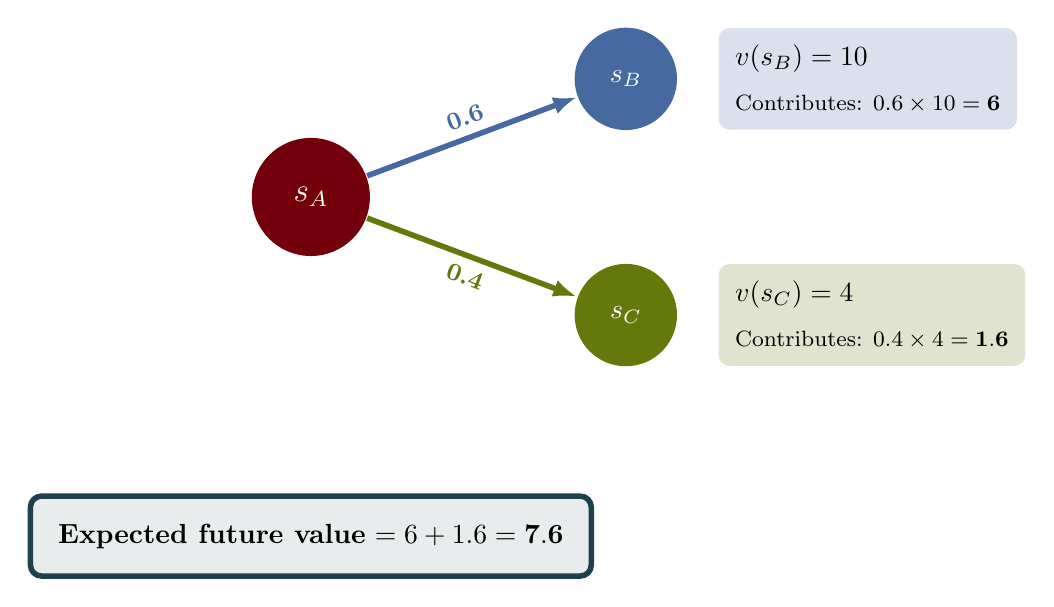
\begin{tikzpicture}[thick]
        % Current state
        \node[circle, fill=Garnet, text=white, minimum size=1.5cm, font=\large] (s) at (0,0) {$s_A$};

        % Future states
        \node[circle, fill=SecondaryBlue, text=white, minimum size=1.3cm] (s1) at (4, 1.5) {$s_B$};
        \node[circle, fill=SecondaryGreen, text=white, minimum size=1.3cm] (s2) at (4, -1.5) {$s_C$};

        % Arrows with calculations
        \draw[-{Latex[length=3mm]}, line width=2pt, SecondaryBlue] (s) -- node[above, sloped, font=\small\bfseries] {0.6} (s1);
        \draw[-{Latex[length=3mm]}, line width=2pt, SecondaryGreen] (s) -- node[below, sloped, font=\small\bfseries] {0.4} (s2);

        % Value and calculation boxes
        \node[right=0.5cm of s1, fill=SecondaryBlue!20, inner sep=6pt, rounded corners, align=left] {$v(s_B) = 10$\\[0.2em]\footnotesize Contributes: $0.6 \times 10 = \mathbf{6}$};
        \node[right=0.5cm of s2, fill=SecondaryGreen!20, inner sep=6pt, rounded corners, align=left] {$v(s_C) = 4$\\[0.2em]\footnotesize Contributes: $0.4 \times 4 = \mathbf{1.6}$};

        % Result
        \node[below=3cm of s, draw=FlatDark, line width=2pt, rounded corners, inner sep=10pt, fill=FlatDark!10] {
            \textbf{Expected future value} $= 6 + 1.6 = \mathbf{7.6}$
        };
    \end{tikzpicture}
    \caption{The ``Backup'' Diagram: Average over all possible next states.}
    \label{fig:backup}
\end{figure}

Mathematically, this is the \textbf{Law of Total Expectation}:
\begin{equation}
    \mathbb{E}[G_{t+1} \mid S_t = s] = \sum_{s'} p(s'|s) \cdot \underbrace{\mathbb{E}[G_{t+1} \mid S_{t+1} = s']}_{\text{value if we land at } s'}
    \label{eq:total_exp}
\end{equation}

\newpage
\subsection{Step 5: Recognize the Recursion}

Look closely at the term $\mathbb{E}[G_{t+1} \mid S_{t+1} = s']$ from Step 4.

\textbf{Question}: What does this represent?

\textbf{Answer}: ``The expected total return starting from time $t+1$, given we're in state $s'$ at time $t+1$.''

\begin{tcolorbox}[memorybox={The Aha! Moment}]
But wait... ``expected total return starting from state $s'$'' is \textbf{exactly the definition of $v(s')$}!

\[ \mathbb{E}[G_{t+1} \mid S_{t+1} = s'] = v(s') \]

\textbf{This is the recursion!} The value of a state depends on the values of neighboring states.
\end{tcolorbox}

Substituting this back into our equation from Step 4:
\begin{equation}
    \mathbb{E}[G_{t+1} \mid S_t = s] = \sum_{s'} p(s'|s) \cdot v(s')
    \label{eq:weighted_future}
\end{equation}

\begin{tcolorbox}[examplebox={Computing Part B for $s_A$}]
Now we can calculate the ``Part B'' we left hanging in Step 3:
\begin{align*}
\mathbb{E}[G_{t+1} \mid S_t = s_A] &= p(s_B|s_A) \cdot v(s_B) + p(s_C|s_A) \cdot v(s_C) \\[0.3em]
&= (0.6)(10) + (0.4)(4) \\[0.3em]
&= 6 + 1.6 \\[0.3em]
&= \mathbf{7.6}
\end{align*}

The expected value of ``wherever I end up next'' is \$7.6.
\end{tcolorbox}

\vspace{1em}
\subsection{Step 6: Put It All Together}

Now we combine everything. From Step 3, we had:
\[ v(s) = r(s) + \gamma \cdot \mathbb{E}[G_{t+1} \mid S_t = s] \]

From Step 5, we found:
\[ \mathbb{E}[G_{t+1} \mid S_t = s] = \sum_{s'} p(s'|s) \cdot v(s') \]

Substituting:

\begin{framed}
\centering
\Large
\textbf{The Bellman Equation}
\[ \boxed{v(s) = r(s) + \gamma \sum_{s'} p(s'|s) \cdot v(s')} \]
\end{framed}

\begin{tcolorbox}[memorybox={The Equation in Plain English}]
\begin{center}
\renewcommand{\arraystretch}{1.5}
\begin{tabular}{rcl}
\textbf{Value of being here} & $=$ & \textbf{What I get now} \\
& $+$ & \textbf{Discounted average of where I might go}
\end{tabular}
\end{center}

\vspace{0.5em}
Or even simpler: \textit{``Today's value = Today's reward + Tomorrow's (discounted) value''}
\end{tcolorbox}

\begin{tcolorbox}[examplebox={Final Answer for $s_A$}]
\begin{align*}
v(s_A) &= r(s_A) + \gamma \cdot \bigl[ p(s_B|s_A) \cdot v(s_B) + p(s_C|s_A) \cdot v(s_C) \bigr] \\[0.5em]
&= \underbrace{5}_{\text{tip now}} + \; 0.9 \times \underbrace{7.6}_{\text{expected future}} \\[0.5em]
&= 5 + 6.84 \\[0.5em]
&= \boxed{\$11.84}
\end{align*}

\textbf{Interpretation}: Standing at location $s_A$, you can expect to earn \$11.84 total (in today's dollars).
\end{tcolorbox}

\newpage
% ==========================================
\section{Part 5: Why This Matters}
% ==========================================

\subsection{The Power of Recursion}

The Bellman equation is \vocab{recursive}: it defines $v(s)$ in terms of $v(s')$ for neighboring states.

\begin{tcolorbox}[memorybox={The Bootstrap Principle}]
\textbf{You don't need to simulate the entire future.}

If someone tells you the value of all neighboring states, you can immediately compute your own value using one simple formula.
\end{tcolorbox}

\subsection{Three Analogies to Remember}

\begin{enumerate}
    \item \textbf{GPS Navigation}: Your estimated arrival time = time to next intersection + ETA from that intersection. The GPS doesn't re-calculate the entire route; it just looks one step ahead.

    \item \textbf{House Prices}: Your home's value = what you could rent it for this month + discounted future rental income. Real estate appraisers use exactly this logic.

    \item \textbf{Career Planning}: Value of your current job = this year's salary + discounted value of where this job leads (promotions, opportunities).
\end{enumerate}

\subsection{The Complete Picture}

\begin{figure}[H]
    \centering
    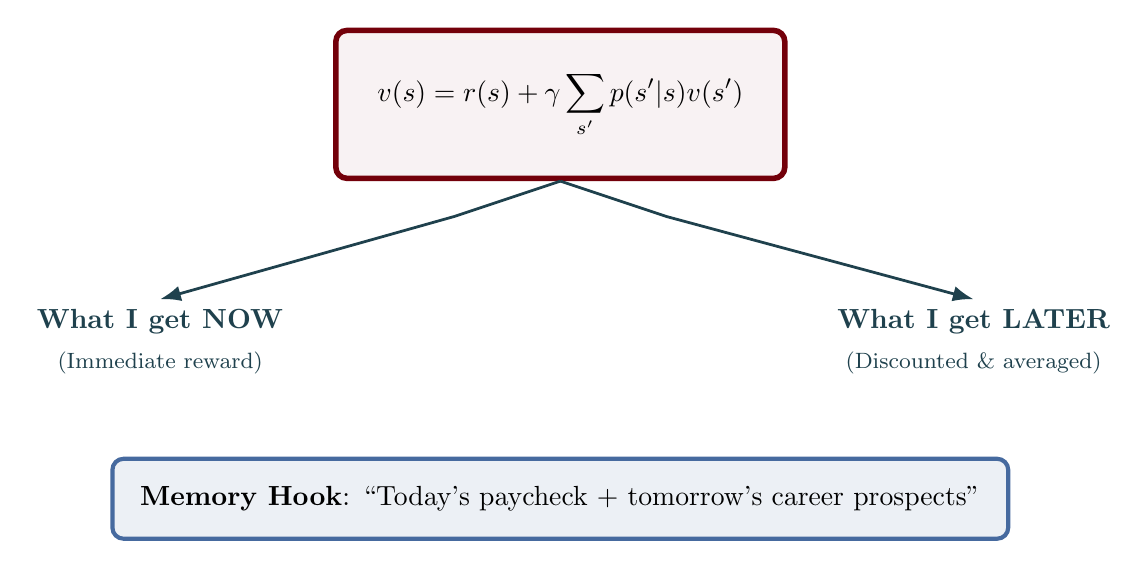
\begin{tikzpicture}[thick, scale=0.9]
        % Main equation box
        \node[draw=Garnet, line width=2pt, rounded corners, inner sep=15pt, fill=Garnet!5] (eq) at (0,0) {
            $v(s) = r(s) + \gamma \displaystyle\sum_{s'} p(s'|s) v(s')$
        };

        % Breakdown arrows
        \node[below left=1.5cm and 0.5cm of eq, align=center, text=FlatDark] (now) {
            \textbf{What I get NOW}\\
            \footnotesize (Immediate reward)
        };
        \node[below right=1.5cm and 0.5cm of eq, align=center, text=FlatDark] (later) {
            \textbf{What I get LATER}\\
            \footnotesize (Discounted \& averaged)
        };

        \draw[-{Latex}, FlatDark, line width=1pt] (eq.south) -- ++(-1.5,-0.5) -- (now.north);
        \draw[-{Latex}, FlatDark, line width=1pt] (eq.south) -- ++(1.5,-0.5) -- (later.north);

        % Memory hook
        \node[below=3.5cm of eq, draw=SecondaryBlue, line width=1.5pt, rounded corners, inner sep=10pt, fill=SecondaryBlue!10] {
            \textbf{Memory Hook}: ``Today's paycheck + tomorrow's career prospects''
        };
    \end{tikzpicture}
    \caption{The Bellman Equation decomposes value into immediate and future components.}
    \label{fig:summary}
\end{figure}

\newpage
% ==========================================
\section{Part 6: Quick Reference}
% ==========================================

\begin{center}
\renewcommand{\arraystretch}{1.8}
\begin{tabular}{|c|l|l|}
\hline
\textbf{Symbol} & \textbf{Name} & \textbf{Pizza Delivery Analogy} \\
\hline
$s$ & State & Your current location \\
$S_t$ & State at time $t$ & Where you are at hour $t$ of your shift \\
$R_{t+1}$ & Reward & The tip you receive after a delivery \\
$r(s)$ & Expected immediate reward & Average tip when delivering from location $s$ \\
$G_t$ & Return & Total tips from now until end of shift \\
$\gamma$ & Discount factor & How much you value future tips vs. now \\
$v(s)$ & Value function & Expected total earnings starting from $s$ \\
$p(s'|s)$ & Transition probability & Chance of going to $s'$ when leaving $s$ \\
\hline
\end{tabular}
\end{center}

\section{Conclusion}

The Bellman Equation tells us something profound:

\begin{tcolorbox}[memorybox={The One Sentence Summary}]
\textbf{The value of where you are} = \textbf{what you get now} + \textbf{discounted average of where you might go next}.
\end{tcolorbox}

This recursive structure is what makes reinforcement learning tractable. Instead of computing infinite futures, we break the problem into manageable one-step lookaheads.

Next time you use a GPS, think about how it estimates your arrival time: it doesn't simulate every possible traffic scenario for your entire route. It just looks at the next segment and trusts that the rest has already been computed. That's the Bellman equation in action.

\end{document}
